\documentclass[12pt]{exam}
\newcommand{\hwnumber}{5}
\newcommand{\hwname}{Binomial Heaps}
\newcommand{\duedate}{\formatdate{13}{10}{\YEAR} by \progDueTime}

\usepackage{../misc/latex/edition}  % Course semester
\usepackage{../misc/latex/c0}       % Listings style for c0
\usepackage{amsmath}
\usepackage{enumerate}
\usepackage[normalem]{ulem}
\usepackage{verbatim}
\usepackage[left=1in, right=1in, top=1in, bottom=1in]{geometry}
\usepackage{graphicx}
\usepackage{hyperref}
\usepackage{tikz}     \usetikzlibrary{shapes}
\usepackage{fancybox}
\usepackage[all]{xy}
\usepackage{wrapfig}
\usepackage{fancyvrb}
\usepackage{datetime}
\usepackage{etoolbox}
\usepackage{calc}
\usepackage[nomessages]{fp}
\usepackage{import}  % Like input and include, but respects subdirectories

\newcommand{\defaultQuestionLocation}{questions}
\newcommand{\inputQuestion}[2][\defaultQuestionLocation/]{%
  \subimport{#1}{#2}
}
% Subdirectories of \defaultQuestionLocation containing code and pictures
\newcommand{\code}{code}
\newcommand{\img}{img}


%%% ic: frontmatter macros
\newcommand{\specialInstructions}{}
\newcommand{\HWNUMBER}
{\ifdefempty{\hwnumber}{__}{%
  \ifnumless{\hwnumber}{10}{0\hwnumber}{\hwnumber}}}
\newcommand{\hwtype}{Written Homework}

%%% ic: 'exam' tweaks
\renewcommand{\half}{.5} % Half points

\newcommand{\Question}[2][]
 {\ifstrempty{#1}
    {\question{\bf #2}}
    {\question[#1]{\bf #2}}
  \immediate\write\rubricfile{}%
  \immediate\write\rubricfile{Question \thequestiontitle:}%
  \immediate\write\rubricfile{==========}
 }

%%% ic: Support for editable PDF
% counter name (some viewers misbehave if always the same)
\newcounter{editable}
\newcommand{\nextField}{\addtocounter{editable}{1}q\arabic{editable}}
\newcommand{\NextField}
 {\makebox[0pt][r]{\scalebox{0.1}{\color{White}\nextField}}}

% Color of edit area
\newcommand{\editAreaColor}{red}
% Single line answer:   \editableLine[extra parameters (optional)]{line width}
\newcommand{\editableLine}[2][]
{\textcolor{\editAreaColor}{%
 \underline{\hspace*{-0.25em}%
 \raisebox{-0.5ex}{%
 \TextField[width=#2, borderwidth=0, #1]{\NextField}}}}%
}
% Single line answer for code:  \editableLine[extra parameters (optional)]{line width}
\newcommand{\editableCodeLine}[2][]
{\textcolor{\editAreaColor}{%
 \underline{%
 \TextField[width=#2, height=1.5ex, borderwidth=0, #1]{\NextField}}}}
% Multiline answer:  \editableLine[extra parameters (optional)]{box height}
\newcommand{\editableBox}[2][]
{\leavevmode\hspace*{-0.1em}%
\TextField[height=#2, width=\linewidth,
           multiline=true, borderwidth=0.1, bordercolor=\editAreaColor,
           #1]{\NextField}}

%%%%% Same answer format as exams
\renewcommand{\rmdefault}{ppl}
\renewcommand{\sfdefault}{phv}
\newcommand{\answerColor}{Blue}

\ifprintanswers
\newcommand{\answer}[2]{\makebox[#1][c]{\color{\answerColor}#2}}
\else
\newcommand{\answer}[2]{\makebox[#1][c]{}\makebox[0pt]{\phantom{|}}}
\fi
\newcommand{\uanswer}[2]{\underline{\answer{#1}{#2}}}


%%% Write rubric snippet.  Usage:
% \RUBRIC
% any multi-line text (including \, #, %, whatever)
% ENDRUBRIC
%% (ENDRUBRIC should be on a line by itself)
\makeatletter
\def\RUBRIC
 {%
  \begingroup
  \let\do\@makeother\dospecials
  \endlinechar=`\^^J
  \@tofile%
 }
\def\ENDRUBRIC{ENDRUBRIC}
\def\@tofile#1^^J{%
  \def\@test{#1}%
  \ifx\@test\ENDRUBRIC
    \immediate\write\rubricfile{}  % End with an empty line
    \expandafter\@firstoftwo
  \else
    \expandafter\@secondoftwo
  \fi
  {\endgroup}%
  {\toks@{#1}%
   \begingroup\endlinechar=\m@ne
   \everyeof{\noexpand}%
   \xdef\@temp{\scantokens\expandafter{\the\toks@}}%
   \endgroup
   \immediate\write\rubricfile{\@temp}%
   \@tofile}%
}
\makeatother

%% Displays tags for an exercise in 'answer' mode
\newcommand{\TAGS}[1]
{\ifprintanswers%
  \rule{0em}{0ex}%
  \marginpar{\footnotesize%
    \fcolorbox{black}{Gray!25}{%
      \parbox[t]{2cm}{\raggedright\textbf{TAGS:}\\#1}}}%
  \ignorespaces%
 \fi}%


%% Page layout
\pagestyle{headandfoot}

\headrule
\header{\textbf{\courseNumber{} \hwtype{} \hwnumber}}
       {}
       {\textbf{Page \thepage\ of \numpages}}
\footrule
\footer{}{}{\COPYRIGHT}

\renewcommand{\partlabel}{\textbf{\thequestion.\thepartno}}
%\renewcommand{\partlabel}{\textbf{Task \thepartno}}
\renewcommand{\subpartlabel}{\textbf{\thesubpart.}}
\renewcommand{\thepartno}{\arabic{partno}}
\renewcommand{\thesubpart}{\alph{subpart}}
\pointpoints{pt}{pts}
\pointformat{\raisebox{0ex}[\height][0pt]{\fcolorbox{black}{yellow}{\themarginpoints}}}
\bonuspointformat{\raisebox{0ex}[\height][0pt]{\fcolorbox{black}{red}{\themarginpoints}}}
\marginpointname{\points}
\pointsinmargin
%\boxedpoints

\setlength\answerlinelength{2in}
\setlength\answerskip{0.3in}

\newcommand{\mkWrittenTitle}[1]{#1}
\newcommand{\mkDueDate}[1]{#1}
\newcommand{\mkEvalSummary}[1]{#1}
\newcommand{\mkGradetable}[1]{#1}



% This fixes an issue with the exam package version 2.6 and after,
% where 'framed' has been renamed to 'examframed' to avoid a conflict.
\ifcsmacro{examframed}{%
\newenvironment{framed}
{\begin{examframed}}
{\end{examframed}}
}{}

\begin{document}
\hwTitle

\noindent
For the programming portion of this week's homework, we'll explore a
variant of the heap data structure, called \emph{binomial
  heaps}. Binomial heaps have two advantages over the heaps we have
discussed in class: first, they have an amortized constant time
insertion operation. Second, it is possible to merge two heaps into a
single heap in $O(\log n)$ time, where $n$ is the number of elements
in the combined heap. The downside of binomial heaps is that they

\bigskip
\noindent
The code handout for this assignment is at
\begin{center}
\whereisthetgz{binomial-handout.tgz}
\end{center}
The file \lstinline'README.txt' in the code handout goes over the contents
of the handout and explains how to hand the assignment in.
There is a FIFTEEN (15) PENALTY-FREE HANDIN LIMIT.
Every additional handin will incur a small (5\%) penalty (even if
using a late day).

\newpage
\section{Binomial trees}

Binomial heaps are made up of \emph{binomial trees}.  Binomial tree
are not the same as binary trees, because parent notes can have more
than two children. Binomial trees are defined recursively as follows:

\begin{itemize}
\item%
  A binomial tree of order 0 (denoted $B_0$) is a single root node.
\item%
  A binomial tree of order k (denoted $B_k$, $k > 0$) consists of a
  root node whose children are roots of binomial trees of orders
  $k-1$, $k-2$, ..., 1, 0 (in that order).
\end{itemize}
Here are pictures of the shapes of $B_0$, $B_1$, $B_2$, $B_3$ (data
not shown):
\begin{center}
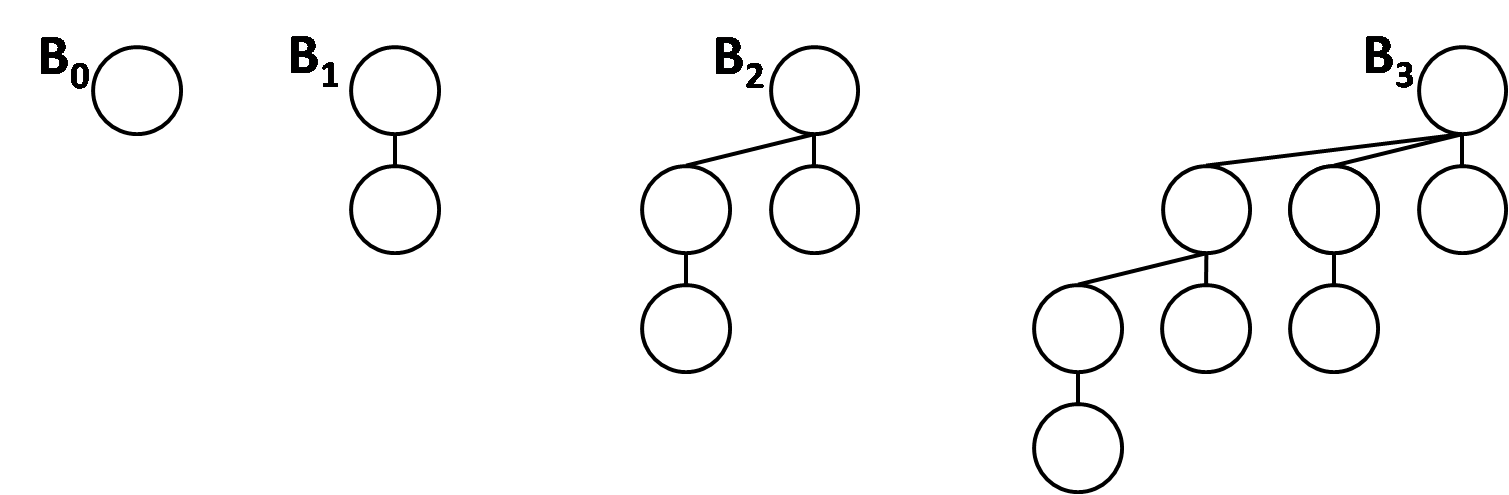
\includegraphics[width=0.9\textwidth]{\img/binheaps.png}
\end{center}

In addition to this shape invariant, we require that the binomial
trees obey the order invariant similar to min-heaps. For example, here
is $B_3$ with keys that obey the order invariant for min-heaps, where
smaller integers have higher priority:
\begin{center}
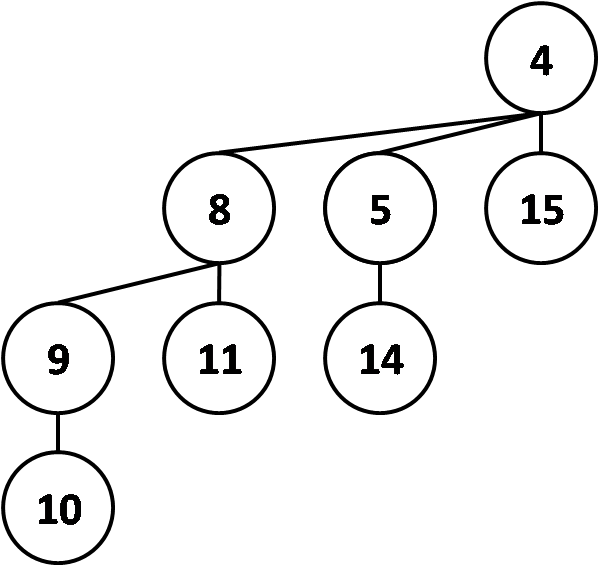
\includegraphics[width=0.3\textwidth]{\img/binheapsB3.png}
\end{center}

In C0/C1, we can represent each node of a binomial tree using a
\lstinline'struct'. Since a node may have more than two children, we
can't store pointers to the children using \lstinline'left' and
\lstinline'right' fields. Instead, we can store a pointer to a node's
leftmost child and a pointer to its next sibling.
%The binomial tree also has a header node to point to the root of the tree.

\begin{lstlisting}[numbers=none]
typedef struct binomial_tree_node binotree;
struct binomial_tree_node {
   elem data;
   binotree* child;     // leftmost child of current node
   binotree* sibling;   // next sibling of current node
};
\end{lstlisting}
%typedef struct binomial_tree_header* binomialtree;
%struct binomial_tree_header {
%   binomialnode* root;
%};

\noindent
Here is the binomial tree of order 3 from the previous page, stored as
a pointer structure:
\begin{center}
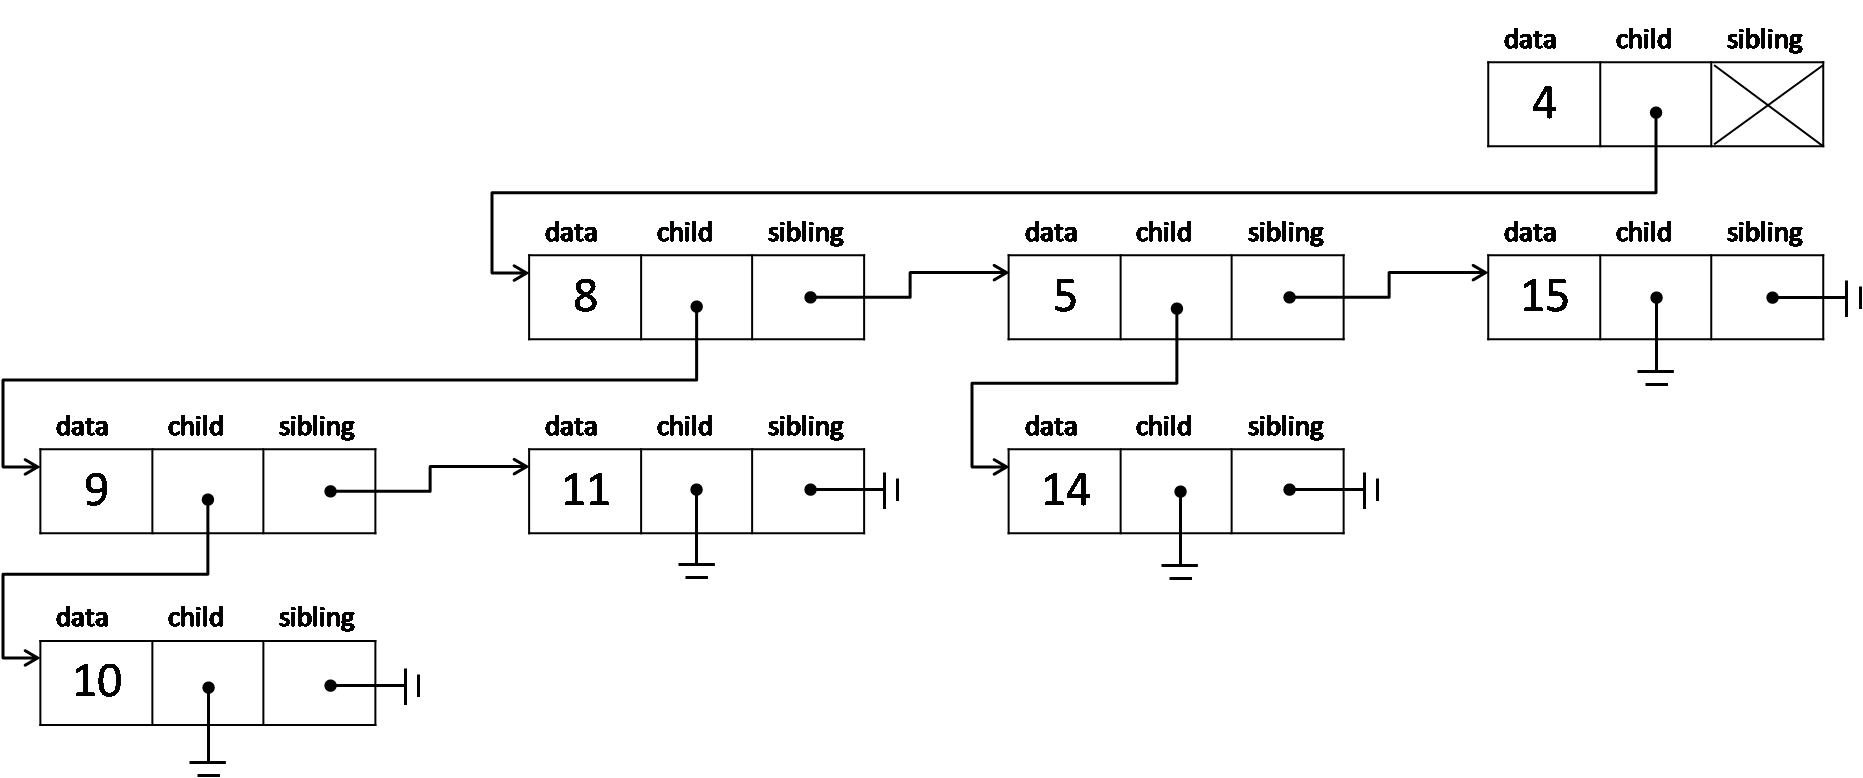
\includegraphics[width=\textwidth]{\img/binheap-pointers.png}
\end{center}
In this assignment, we will be implementing the interface of generic
priority queues using binomial heaps. Therefore, the picture above is
somewhat incorrect: the data in our priority queues will always have
type \lstinline'void*'. Therefore, the data fields could not possibly
contain integers directly: at best they could contain pointers to
those integers which had been cast to \lstinline'void*'.

\begin{task}[3]
  In the file \lstinline'bheap.c1', finish the implementation of the
  specification function \lstinline'is_binotree(T, k, hi_pri)'. This
  function should return true exactly when \lstinline'T' is a binomial
  tree of order \lstinline'k' implemented by the strategy above. The
  function pointer \lstinline'(*hi_pri)(x,y)' returns true when
  \lstinline'x' has strictly higher priority than \lstinline'y'.
\end{task}

A critical feature of binomial trees is that two binomial trees of
order $k$ can be merged into a single binomial tree of order $k+1$ in
constant time without allocating any extra memory.
As an example, the merge of the following two binomial trees of order
2 on the left results in the binomial tree of order 3 on the right:
\begin{center}
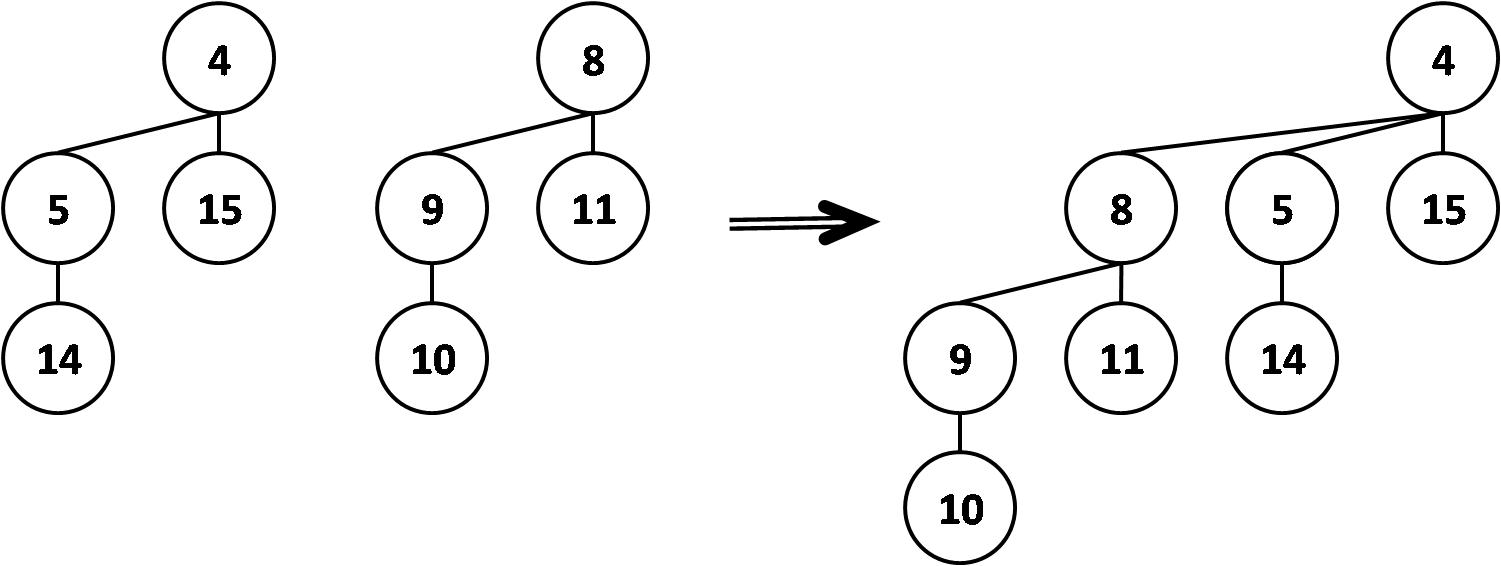
\includegraphics[width=0.8\textwidth]{\img/binheap-merge.png}
\end{center}

\begin{task}[3]
  In the file \lstinline'bheap.c1', finish the implementation of the
  constant-time function \lstinline'binotree_merge(T1, T2, k, hi_pri)'
  which merges \lstinline'T1' and \lstinline'T2', binomial trees of
  order \lstinline'k', into a single binomial tree of order
  \lstinline'k+1'. The resulting tree must obey the heap ordering
  invariant according to the \lstinline'hi_pri' function pointer.
\end{task}

\section{Binomial heaps}

A binomial heap is a collection of binomial trees where there is at
most one tree of each order. We use binomial heaps to implement the
same priority interface that we implemented in class:

\begin{quote}
\begin{lstlisting}
// typedef ______* bheap_t;

bool bheap_empty(bheap_t H)
  /*@requires H != NULL; @*/ ;
bheap_t bheap_new(higher_priority_fn* hi_pri)
  /*@requires hi_pri != NULL; @*/
  /*@ensures \result != NULL && bheap_empty(\result); @*/ ;
void bheap_add(bheap_t H, elem x)
  /*@requires !bheap_full(H); @*/ ;
elem bheap_rem(bheap_t H)
  /*@requires !bheap_empty(H); @*/ ;
\end{lstlisting}
\end{quote}

We have already given you implementations of these four fucntions, but
three of these four functions depend on four functions that you need
to write. These four functions operate on the type
\lstinline'binolist*', linked lists where the first element contains
either \lstinline'NULL' or a tree $B_0$, the second element contains
either \lstinline'NULL' or a tree $B_1$, and so on. We give you the
data structure invariant for these linked lists in
\lstinline'binolist*':

\begin{quote}
\begin{lstlisting}[numbers=none]
struct binomial_listnode binolist;
struct binomial_listnode {
  binotree* tree;
  binolist* next;
};

bool is_binolist(binolist* L, int k, higher_priority_fn* hi_pri) {
  if (L == NULL) return true;
  return (L->tree == NULL || is_binotree(L, k, hi_pri))
    && is_binolist(L->next, k+1, hi_pri);
}
\end{lstlisting}
\end{quote}

One consequence of this data structure invariant is that you could
potentially have a long linked list which contained only
\lstinline'NULL' without there being any tree at the end. This makes
it somewhat more expensive to check whether a binary heap is empty or
not.

A binomial tree


you will
implement the data structure of ropes, which provide


\end{document}
